% Options for packages loaded elsewhere
\PassOptionsToPackage{unicode}{hyperref}
\PassOptionsToPackage{hyphens}{url}
%
\documentclass[
]{article}
\usepackage{amsmath,amssymb}
\usepackage{iftex}
\ifPDFTeX
  \usepackage[T1]{fontenc}
  \usepackage[utf8]{inputenc}
  \usepackage{textcomp} % provide euro and other symbols
\else % if luatex or xetex
  \usepackage{unicode-math} % this also loads fontspec
  \defaultfontfeatures{Scale=MatchLowercase}
  \defaultfontfeatures[\rmfamily]{Ligatures=TeX,Scale=1}
\fi
\usepackage{lmodern}
\ifPDFTeX\else
  % xetex/luatex font selection
    \setmainfont[]{Arial}
\fi
% Use upquote if available, for straight quotes in verbatim environments
\IfFileExists{upquote.sty}{\usepackage{upquote}}{}
\IfFileExists{microtype.sty}{% use microtype if available
  \usepackage[]{microtype}
  \UseMicrotypeSet[protrusion]{basicmath} % disable protrusion for tt fonts
}{}
\makeatletter
\@ifundefined{KOMAClassName}{% if non-KOMA class
  \IfFileExists{parskip.sty}{%
    \usepackage{parskip}
  }{% else
    \setlength{\parindent}{0pt}
    \setlength{\parskip}{6pt plus 2pt minus 1pt}}
}{% if KOMA class
  \KOMAoptions{parskip=half}}
\makeatother
\usepackage{xcolor}
\usepackage[landscape,top=5cm,left=2.5cm,bottom=2cm,right=2.5cm,margin=1in]{geometry}
\usepackage{graphicx}
\makeatletter
\def\maxwidth{\ifdim\Gin@nat@width>\linewidth\linewidth\else\Gin@nat@width\fi}
\def\maxheight{\ifdim\Gin@nat@height>\textheight\textheight\else\Gin@nat@height\fi}
\makeatother
% Scale images if necessary, so that they will not overflow the page
% margins by default, and it is still possible to overwrite the defaults
% using explicit options in \includegraphics[width, height, ...]{}
\setkeys{Gin}{width=\maxwidth,height=\maxheight,keepaspectratio}
% Set default figure placement to htbp
\makeatletter
\def\fps@figure{htbp}
\makeatother
\setlength{\emergencystretch}{3em} % prevent overfull lines
\providecommand{\tightlist}{%
  \setlength{\itemsep}{0pt}\setlength{\parskip}{0pt}}
\setcounter{secnumdepth}{-\maxdimen} % remove section numbering
\usepackage{graphicx}
\usepackage{xcolor}
\usepackage{eso-pic}
\usepackage{lipsum}
\definecolor{azuloscuro}{RGB}{0,51,102}
\definecolor{turquesa}{RGB}{0,174,239}
\usepackage{fancyhdr}
\pagestyle{fancy}
\fancyhf{}
\renewcommand{\headrulewidth}{0pt}
\fancyfoot[R]{\thepage}
\usepackage{booktabs}
\usepackage{longtable}
\usepackage{array}
\usepackage{multirow}
\usepackage{wrapfig}
\usepackage{float}
\usepackage{colortbl}
\usepackage{pdflscape}
\usepackage{tabu}
\usepackage{threeparttable}
\usepackage{threeparttablex}
\usepackage[normalem]{ulem}
\usepackage{makecell}
\usepackage{xcolor}
\ifLuaTeX
  \usepackage{selnolig}  % disable illegal ligatures
\fi
\usepackage{bookmark}
\IfFileExists{xurl.sty}{\usepackage{xurl}}{} % add URL line breaks if available
\urlstyle{same}
\hypersetup{
  hidelinks,
  pdfcreator={LaTeX via pandoc}}

\author{}
\date{\vspace{-2.5em}2025-04-21}

\begin{document}

\thispagestyle{empty}

\AddToShipoutPictureBG*{
  
\includegraphics[width=\paperwidth,height=\paperheight]{image.png}
}

\vspace*{6cm}

\begin{flushleft}
  {\fontsize{38}{45}\selectfont \textbf{\textcolor{white}{Flood Model Report}}} \\[0.8cm]
  {\fontsize{24}{30}\selectfont \textcolor{white}{Portfolio Analysis}} \\[1.2cm]
  {\fontsize{24}{30}\selectfont \textcolor{white}{Cliente ABC}} \\[0.4cm]
  {\Large \textcolor{white}{Abril 2025}} \\[4cm]
  {\small \textcolor{white}{A business of XXX}}
\end{flushleft}

\noindent \textbf{\textcolor{turquesa}{\fontsize{16}{20}\selectfont Contenido}}

\noindent

\begin{enumerate}
  \item {\fontsize{11}{13}\selectfont Summary \dotfill \pageref{sec:summary}}
  \item {\fontsize{11}{13}\selectfont Results \dotfill \pageref{sec:results}}
\end{enumerate}

\newpage

\noindent \textbf{\textcolor{turquesa}{\fontsize{16}{20}\selectfont Considerations}}
\vspace{0.5cm}

\noindent \fontsize{11}{13}\selectfont The technology used and the
references provided for the generation of this information are based on
scientific data, mathematical models, and encoded experience from
researchers and specialists in the field of Data Management.

\begin{itemize}
  \item {\fontsize{11}{13}\selectfont The present report, as well as the analysis, models,    and predictions contained in this document ("Information", are based on data provided by    MARSH through our client: Cliente ABC and managed through the risk         assessment computer technology owned by JBA Risk Management.}
  \item {\fontsize{11}{13}\selectfont It is important to mention that the accuracy of the     predictions depends largely on the accuracy and quality of the data provided by the         client: Cliente ABC to the MARSH specialists}
  \item {\fontsize{11}{13}\selectfont The management of the information provided by Cliente ABC is carried out through the licensing of MARSH in JBA Risk             Management, using regulatory frameworks for the protection of confidential information,     prohibiting its distribution to third parties without the prior written consent of MARSH    and JBA Risk Management.}
  \item {\fontsize{11}{13}\selectfont The information described within the report generated   by Marsh can only be used for the purpose of studying and interpreting results for Cliente ABC. This document cannot be used under any circumstances in the          development and/or calibration of any product or service offerings that competi with JBA    Risk Management and MARSH..}
\end{itemize}

\fontsize{11}{13}\selectfont The global flood maps from JBA Risk
Management, and the information management from Marsh, provide
indicative information about the extent and depth of flooding for
undefended rivers and surface water flood risks for return periods of
20, 50, 100, 200, 500, and 1,500 years.The underlying digital elevation
data is a combination of Digital Terrain Models (DTMs) from a variety of
sources.

\fontsize{11}{13}\selectfont For post-2020 map updates, Airbus
WorldDEM's DTMlite is widely used. When MDT is not available, Intermap
Technologies Inc.'s NEXTMAP World 30 Digital Surface Model (DSM) is
used. Flood risk mapping is provided globally at a resolution of 30m for
all rivers and surface waters. The maps are created by simulating design
rainfall totals and river flow volumes, allowing the associated flooding
to spread across the surrounding terrain using hydraulic modeling
software. In order to estimate river flows and rainfall amounts for each
return period anywhere in the world, JBA has developed suitable
hydrological models for global-scale mapping.

\newpage

\noindent \textbf{\textcolor{azuloscuro}{\fontsize{28}{32}\selectfont Summary}}
\label{sec:summary} \vspace{0.5cm}

\fontsize{11}{13}\selectfont This probabilistic report serves as a tool
to assess and quantify your flood risk. This analysis uses mathematical
and statistical models to simulate different flood scenarios and
determine the probability of their occurrence at a given time.
Historical, topographic, and precipitation data are used to create this
report for specific areas. The results are presented for return periods
of 20, 50, 100, 200, 500, and 1500 years, showing the affected areas and
their extent.

\fontsize{11}{13}\selectfont The purpose of this report is to provide
Cliente ABC with a Flood Risk Assessment.

\fontsize{11}{13}\selectfont The scope of the project includes directly
importing input data, as provided by the client, into the model and
running the analyses. The JBA Global Flood Event Set allows for
examining flood patterns and assessing regional, continental, and global
exposures for Cliente ABC. The model utilizes sophisticated statistical
methods, along with physical rainfall and runoff modeling processes, to
capture potential spatial and temporal correlations of floods caused by
tropical cyclones, extreme precipitation, and river discharge.
Hydrological accumulation zones are used to better understand flood
correlations and identify areas that may be simultaneously affected by
the same event, providing an alternative geographic unit for aggregation
and accumulation analysis beyond political administrative boundaries.
River flood results represent floods caused by any moving water (rivers,
streams, drains). Surface water results represent floods caused by water
stagnation and overflow of water bodies deposited in depressions of the
terrain.

\fontsize{11}{13}\selectfont The country-level catastrophic models of
JBA incorporate their high-resolution flood data and internationally
recognized climate projections, allowing for the assessment of current
baseline and future risk of river and surface water flooding with
confidence for all countries worldwide.

\fontsize{11}{13}\selectfont The results provided by this report are
important for making decisions regarding land use prevention,
infrastructure construction, and post-flood recovery planning. It is
recommended to take preventive and mitigation measures to reduce the
impact of floods and protect human life, property, and infrastructure,
as well as to consider it in order to safeguard machinery, supplies, or
important inventories that may cause total or partial business
interruption.

\newpage

\noindent \textbf{\textcolor{azuloscuro}{\fontsize{11}{13}\selectfont The following considerations were considered for Cliente ABC:}}
\vspace{0.5cm}

\begin{table}[!h]
\centering\begingroup\fontsize{11}{13}\selectfont

\resizebox{\ifdim\width>\linewidth\linewidth\else\width\fi}{!}{
\begin{tabular}{cccccc}
\toprule
\cellcolor{azuloscuro}{\textcolor{white}{ID}} & \cellcolor{azuloscuro}{\textcolor{white}{Name}} & \cellcolor{azuloscuro}{\textcolor{white}{Country}} & \cellcolor{azuloscuro}{\textcolor{white}{Latitude}} & \cellcolor{azuloscuro}{\textcolor{white}{Longitude}} & \cellcolor{azuloscuro}{\textcolor{white}{Buffer}}\\
\midrule
\cellcolor{gray!10}{1} & \cellcolor{gray!10}{Centro ABC} & \cellcolor{gray!10}{Dominican Republic} & \cellcolor{gray!10}{18.52248} & \cellcolor{gray!10}{-69.74553} & \cellcolor{gray!10}{Polygon}\\
2 & Centro xyz & Dominican Republic & 18.52779 & -69.83790 & Polygon\\
\bottomrule
\end{tabular}}
\endgroup{}
\end{table}

\vspace{1cm}

\begin{table}[!h]
\centering
\begin{tabular}{lll}
\toprule
\multicolumn{1}{>{\centering\arraybackslash}m{0.3\textwidth}}{\cellcolor{azuloscuro}{\color{white}\textbf{Centro 2SDF}}} & \multicolumn{1}{>{\centering\arraybackslash}m{0.3\textwidth}}{\cellcolor{azuloscuro}{\color{white}\textbf{Centro 2SDF3}}} & \multicolumn{1}{>{\centering\arraybackslash}m{0.3\textwidth}}{\cellcolor{azuloscuro}{\color{white}\textbf{Centro 3ABC}}}\\
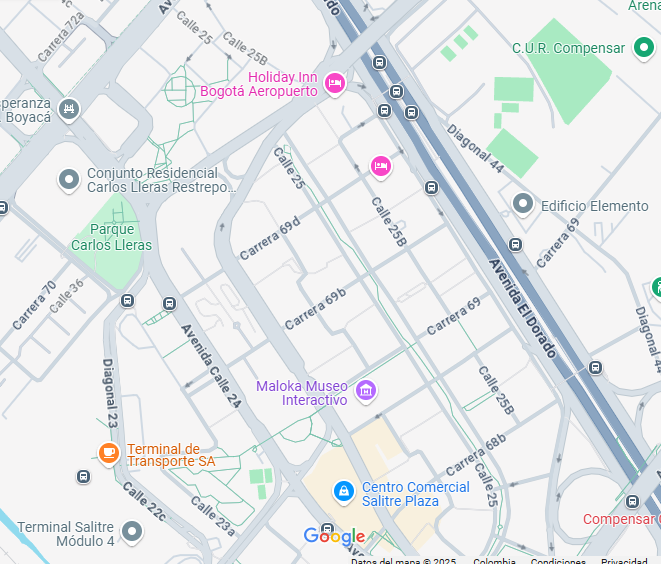
\includegraphics[width=0.3\textwidth]{temp_maps/Centro 2SDF.png} & 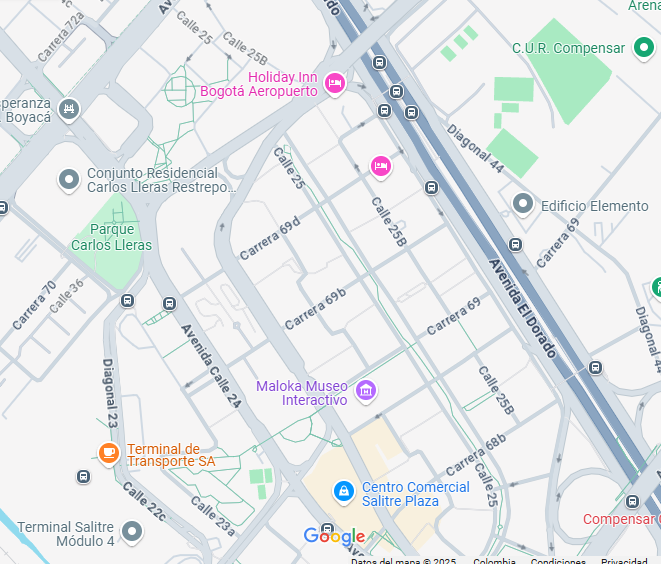
\includegraphics[width=0.3\textwidth]{temp_maps/Centro 2SDF3.png} & 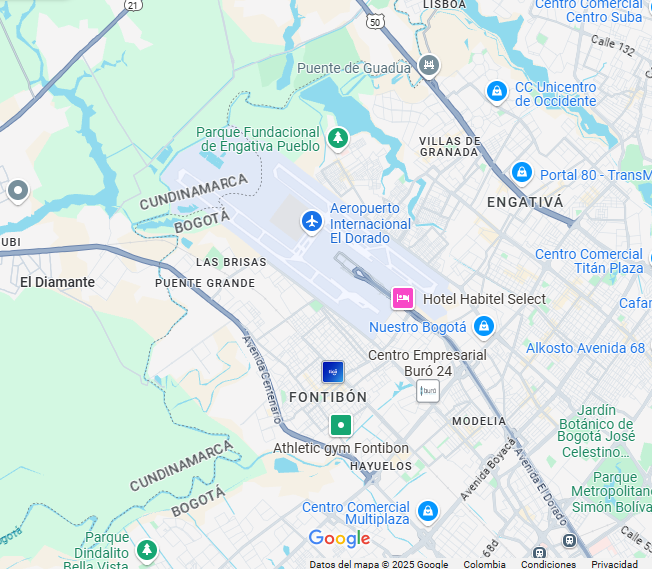
\includegraphics[width=0.3\textwidth]{temp_maps/Centro 3ABC.png}\\
\bottomrule
\end{tabular}
\end{table}
\vspace{0.8cm}
\newpage
\vspace*{\fill}
\begin{table}[!h]
\centering
\begin{tabular}{lll}
\toprule
\multicolumn{1}{>{\centering\arraybackslash}m{0.3\textwidth}}{\cellcolor{azuloscuro}{\color{white}\textbf{Centro ABC}}} & \multicolumn{1}{>{\centering\arraybackslash}m{0.3\textwidth}}{\cellcolor{azuloscuro}{\color{white}\textbf{Centro ABC3}}} & \\
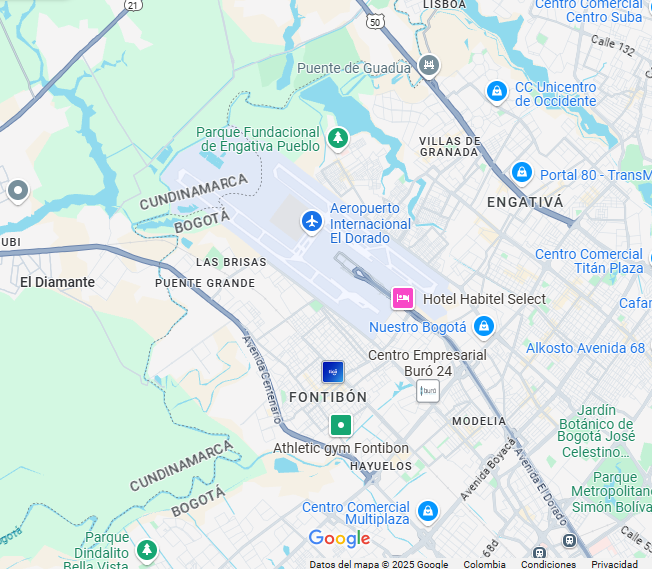
\includegraphics[width=0.3\textwidth]{temp_maps/Centro ABC.png} & 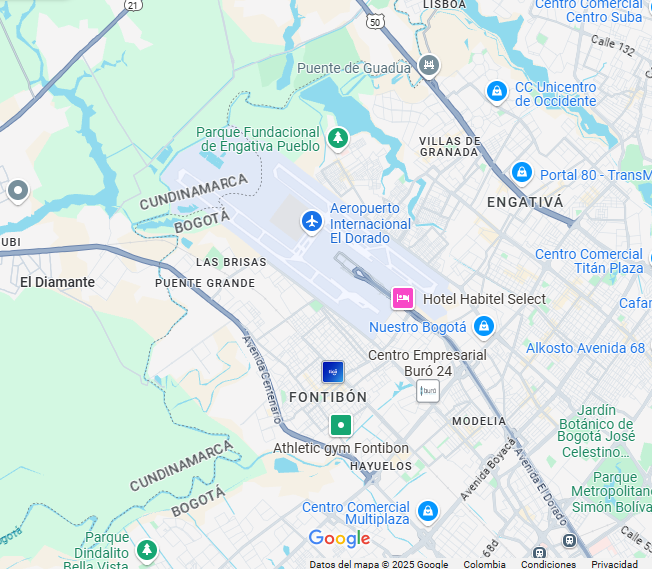
\includegraphics[width=0.3\textwidth]{temp_maps/Centro ABC3.png} & \\
\bottomrule
\end{tabular}
\end{table}
\vspace*{\fill}

\newpage

\noindent \textbf{\textcolor{azuloscuro}{\fontsize{28}{32}\selectfont Results}}
\label{sec:results}

\vspace{0.5cm}

\textbf{\textcolor{turquesa}{\fontsize{16}{20}\selectfont Centro ABC}}

\vspace{0.5cm}

\fontsize{11}{13}\selectfont The following table shows the average and
maximum flood in meters for the location Centro ABC.

\vspace{1cm}

\begin{table}[!h]
\centering\begingroup\fontsize{11}{13}\selectfont

\resizebox{\ifdim\width>\linewidth\linewidth\else\width\fi}{!}{
\begin{tabular}{cccccccc}
\toprule
\multicolumn{2}{c}{\cellcolor{azuloscuro}{\textcolor{white}{Periodo de Retorno}}} & \multicolumn{3}{c}{\cellcolor{azuloscuro}{\textcolor{white}{Profundidad Inundación Ríos}}} & \multicolumn{3}{c}{\cellcolor{azuloscuro}{\textcolor{white}{Profundidad Aguas Superficiales}}} \\
\cmidrule(l{3pt}r{3pt}){1-2} \cmidrule(l{3pt}r{3pt}){3-5} \cmidrule(l{3pt}r{3pt}){6-8}
\cellcolor{azuloscuro}{\textcolor{white}{Año}} & \cellcolor{azuloscuro}{\textcolor{white}{Probabilidad}} & \cellcolor{azuloscuro}{\textcolor{white}{Área Afectada (\%)}} & \cellcolor{azuloscuro}{\textcolor{white}{Promedio (m)}} & \cellcolor{azuloscuro}{\textcolor{white}{Máxima (m)}} & \cellcolor{azuloscuro}{\textcolor{white}{Área Afectada  (\%)}} & \cellcolor{azuloscuro}{\textcolor{white}{Promedio  (m)}} & \cellcolor{azuloscuro}{\textcolor{white}{Máxima  (m)}}\\
\midrule
\cellcolor{gray!10}{20} & \cellcolor{gray!10}{1\%} & \cellcolor{gray!10}{20} & \cellcolor{gray!10}{20} & \cellcolor{gray!10}{20} & \cellcolor{gray!10}{20} & \cellcolor{gray!10}{20} & \cellcolor{gray!10}{20}\\
50 & 10\% & 50 & 50 & 50 & 50 & 50 & 50\\
\cellcolor{gray!10}{100} & \cellcolor{gray!10}{1\%} & \cellcolor{gray!10}{100} & \cellcolor{gray!10}{100} & \cellcolor{gray!10}{100} & \cellcolor{gray!10}{100} & \cellcolor{gray!10}{100} & \cellcolor{gray!10}{100}\\
200 & 10\% & 200 & 200 & 200 & 200 & 200 & 200\\
\cellcolor{gray!10}{500} & \cellcolor{gray!10}{1\%} & \cellcolor{gray!10}{500} & \cellcolor{gray!10}{500} & \cellcolor{gray!10}{500} & \cellcolor{gray!10}{500} & \cellcolor{gray!10}{500} & \cellcolor{gray!10}{500}\\
\addlinespace
1500 & 10\% & 1500 & 1500 & 1500 & 1500 & 1500 & 1500\\
\bottomrule
\end{tabular}}
\endgroup{}
\end{table}
\newpage

\textbf{\textcolor{turquesa}{\fontsize{16}{20}\selectfont Centro SDF}}

\vspace{0.5cm}

\fontsize{11}{13}\selectfont The following table shows the average and
maximum flood in meters for the location Centro SDF.

\vspace{1cm}

\begin{table}[!h]
\centering\begingroup\fontsize{11}{13}\selectfont

\resizebox{\ifdim\width>\linewidth\linewidth\else\width\fi}{!}{
\begin{tabular}{cccccccc}
\toprule
\multicolumn{2}{c}{\cellcolor{azuloscuro}{\textcolor{white}{Periodo de Retorno}}} & \multicolumn{3}{c}{\cellcolor{azuloscuro}{\textcolor{white}{Profundidad Inundación Ríos}}} & \multicolumn{3}{c}{\cellcolor{azuloscuro}{\textcolor{white}{Profundidad Aguas Superficiales}}} \\
\cmidrule(l{3pt}r{3pt}){1-2} \cmidrule(l{3pt}r{3pt}){3-5} \cmidrule(l{3pt}r{3pt}){6-8}
\cellcolor{azuloscuro}{\textcolor{white}{Año}} & \cellcolor{azuloscuro}{\textcolor{white}{Probabilidad}} & \cellcolor{azuloscuro}{\textcolor{white}{Área Afectada (\%)}} & \cellcolor{azuloscuro}{\textcolor{white}{Promedio (m)}} & \cellcolor{azuloscuro}{\textcolor{white}{Máxima (m)}} & \cellcolor{azuloscuro}{\textcolor{white}{Área Afectada  (\%)}} & \cellcolor{azuloscuro}{\textcolor{white}{Promedio  (m)}} & \cellcolor{azuloscuro}{\textcolor{white}{Máxima  (m)}}\\
\midrule
\cellcolor{gray!10}{20} & \cellcolor{gray!10}{1\%} & \cellcolor{gray!10}{20} & \cellcolor{gray!10}{340} & \cellcolor{gray!10}{4230} & \cellcolor{gray!10}{230} & \cellcolor{gray!10}{320} & \cellcolor{gray!10}{320}\\
50 & 10\% & 50 & 4530 & 4530 & 530 & 350 & 350\\
\cellcolor{gray!10}{100} & \cellcolor{gray!10}{1\%} & \cellcolor{gray!10}{100} & \cellcolor{gray!10}{4100} & \cellcolor{gray!10}{4130} & \cellcolor{gray!10}{1300} & \cellcolor{gray!10}{3100} & \cellcolor{gray!10}{3100}\\
200 & 10\% & 200 & 4300 & 4300 & 3200 & 3200 & 3200\\
\cellcolor{gray!10}{500} & \cellcolor{gray!10}{1\%} & \cellcolor{gray!10}{500} & \cellcolor{gray!10}{4300} & \cellcolor{gray!10}{4300} & \cellcolor{gray!10}{3500} & \cellcolor{gray!10}{3500} & \cellcolor{gray!10}{3500}\\
\addlinespace
1500 & 10\% & 1500 & 43500 & 13500 & 31500 & 31500 & 13500\\
\bottomrule
\end{tabular}}
\endgroup{}
\end{table}
\newpage

\textbf{\textcolor{turquesa}{\fontsize{16}{20}\selectfont Centro XYZ}}

\vspace{0.5cm}

\fontsize{11}{13}\selectfont The following table shows the average and
maximum flood in meters for the location Centro XYZ.

\vspace{1cm}

\begin{table}[!h]
\centering\begingroup\fontsize{11}{13}\selectfont

\resizebox{\ifdim\width>\linewidth\linewidth\else\width\fi}{!}{
\begin{tabular}{cccccccc}
\toprule
\multicolumn{2}{c}{\cellcolor{azuloscuro}{\textcolor{white}{Periodo de Retorno}}} & \multicolumn{3}{c}{\cellcolor{azuloscuro}{\textcolor{white}{Profundidad Inundación Ríos}}} & \multicolumn{3}{c}{\cellcolor{azuloscuro}{\textcolor{white}{Profundidad Aguas Superficiales}}} \\
\cmidrule(l{3pt}r{3pt}){1-2} \cmidrule(l{3pt}r{3pt}){3-5} \cmidrule(l{3pt}r{3pt}){6-8}
\cellcolor{azuloscuro}{\textcolor{white}{Año}} & \cellcolor{azuloscuro}{\textcolor{white}{Probabilidad}} & \cellcolor{azuloscuro}{\textcolor{white}{Área Afectada (\%)}} & \cellcolor{azuloscuro}{\textcolor{white}{Promedio (m)}} & \cellcolor{azuloscuro}{\textcolor{white}{Máxima (m)}} & \cellcolor{azuloscuro}{\textcolor{white}{Área Afectada  (\%)}} & \cellcolor{azuloscuro}{\textcolor{white}{Promedio  (m)}} & \cellcolor{azuloscuro}{\textcolor{white}{Máxima  (m)}}\\
\midrule
\cellcolor{gray!10}{20} & \cellcolor{gray!10}{1\%} & \cellcolor{gray!10}{20} & \cellcolor{gray!10}{30} & \cellcolor{gray!10}{230} & \cellcolor{gray!10}{230} & \cellcolor{gray!10}{320} & \cellcolor{gray!10}{320}\\
50 & 10\% & 50 & 530 & 530 & 530 & 350 & 350\\
\cellcolor{gray!10}{100} & \cellcolor{gray!10}{1\%} & \cellcolor{gray!10}{100} & \cellcolor{gray!10}{1300} & \cellcolor{gray!10}{1300} & \cellcolor{gray!10}{1300} & \cellcolor{gray!10}{3100} & \cellcolor{gray!10}{3100}\\
200 & 10\% & 200 & 2300 & 2300 & 3200 & 3200 & 3200\\
\cellcolor{gray!10}{500} & \cellcolor{gray!10}{1\%} & \cellcolor{gray!10}{500} & \cellcolor{gray!10}{5300} & \cellcolor{gray!10}{5300} & \cellcolor{gray!10}{3500} & \cellcolor{gray!10}{3500} & \cellcolor{gray!10}{3500}\\
\addlinespace
1500 & 10\% & 1500 & 13500 & 13500 & 31500 & 31500 & 13500\\
\bottomrule
\end{tabular}}
\endgroup{}
\end{table}

\newpage

\newpage

\textbf{\textcolor{turquesa}{\fontsize{16}{20}\selectfont Return Periods – Centro ABC}}

\vspace{0.3cm}
\begin{table}[!h]
\centering
\begin{tabular}{lll}
\toprule
\multicolumn{1}{>{\centering\arraybackslash}m{0.3\textwidth}}{\cellcolor{azuloscuro}{\color{white}\textbf{1-20}}} & \multicolumn{1}{>{\centering\arraybackslash}m{0.3\textwidth}}{\cellcolor{azuloscuro}{\color{white}\textbf{1-50}}} & \multicolumn{1}{>{\centering\arraybackslash}m{0.3\textwidth}}{\cellcolor{azuloscuro}{\color{white}\textbf{1-100}}}\\
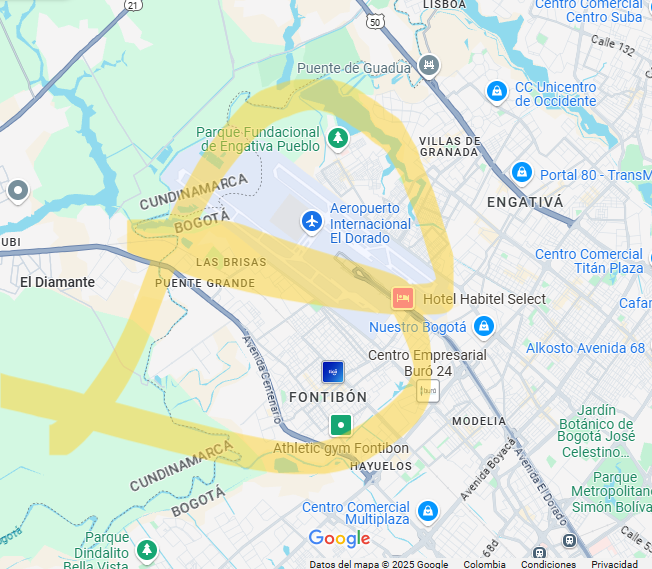
\includegraphics[width=0.3\textwidth]{C:/Users/windows/Documents/GitHub/Problem_Set_1/Flood Report/Flood/1. Mapas/Cliente ABC/Centro ABC/1-20.png} & 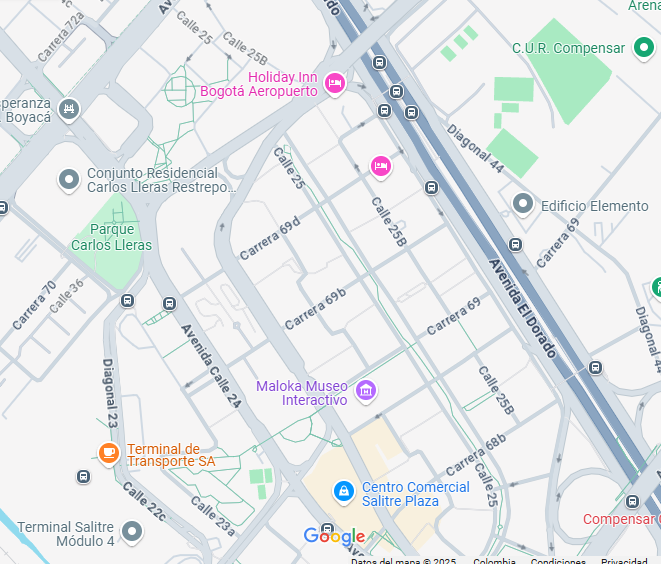
\includegraphics[width=0.3\textwidth]{C:/Users/windows/Documents/GitHub/Problem_Set_1/Flood Report/Flood/1. Mapas/Cliente ABC/Centro ABC/1-50.png} & \includegraphics[width=0.3\textwidth]{C:/Users/windows/Documents/GitHub/Problem_Set_1/Flood Report/Flood/1. Mapas/Cliente ABC/Centro ABC/1-100.png}\\
\bottomrule
\end{tabular}
\end{table}

\vspace{0.5cm}

\begin{table}[!h]
\centering
\begin{tabular}{lll}
\toprule
\multicolumn{1}{>{\centering\arraybackslash}m{0.3\textwidth}}{\cellcolor{azuloscuro}{\color{white}\textbf{1-200}}} & \multicolumn{1}{>{\centering\arraybackslash}m{0.3\textwidth}}{\cellcolor{azuloscuro}{\color{white}\textbf{1-500}}} & \\
\includegraphics[width=0.3\textwidth]{C:/Users/windows/Documents/GitHub/Problem_Set_1/Flood Report/Flood/1. Mapas/Cliente ABC/Centro ABC/1-200.png} & \includegraphics[width=0.3\textwidth]{C:/Users/windows/Documents/GitHub/Problem_Set_1/Flood Report/Flood/1. Mapas/Cliente ABC/Centro ABC/1-500.png} & \\
\bottomrule
\end{tabular}
\end{table}

\vspace{0.5cm}

\newpage

\textbf{\textcolor{turquesa}{\fontsize{16}{20}\selectfont Return Periods – Centro XYZ}}

\vspace{0.3cm}
\begin{table}[!h]
\centering
\begin{tabular}{lll}
\toprule
\multicolumn{1}{>{\centering\arraybackslash}m{0.3\textwidth}}{\cellcolor{azuloscuro}{\color{white}\textbf{1-100}}} & \multicolumn{1}{>{\centering\arraybackslash}m{0.3\textwidth}}{\cellcolor{azuloscuro}{\color{white}\textbf{1-200}}} & \multicolumn{1}{>{\centering\arraybackslash}m{0.3\textwidth}}{\cellcolor{azuloscuro}{\color{white}\textbf{1-500}}}\\
\includegraphics[width=0.3\textwidth]{C:/Users/windows/Documents/GitHub/Problem_Set_1/Flood Report/Flood/1. Mapas/Cliente ABC/Centro XYZ/1-100.png} & \includegraphics[width=0.3\textwidth]{C:/Users/windows/Documents/GitHub/Problem_Set_1/Flood Report/Flood/1. Mapas/Cliente ABC/Centro XYZ/1-200.png} & \includegraphics[width=0.3\textwidth]{C:/Users/windows/Documents/GitHub/Problem_Set_1/Flood Report/Flood/1. Mapas/Cliente ABC/Centro XYZ/1-500.png}\\
\bottomrule
\end{tabular}
\end{table}

\vspace{0.5cm}

\begin{table}[!h]
\centering
\begin{tabular}{lll}
\toprule
\multicolumn{1}{>{\centering\arraybackslash}m{0.3\textwidth}}{\cellcolor{azuloscuro}{\color{white}\textbf{1-1500}}} &  & \\
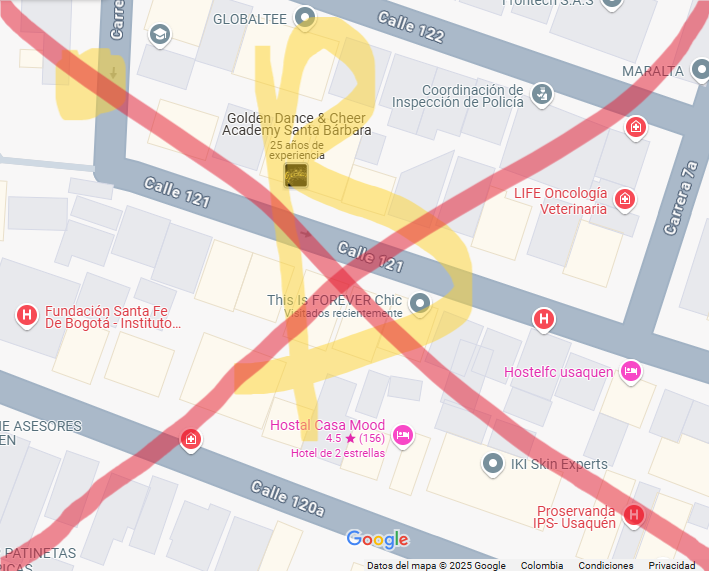
\includegraphics[width=0.3\textwidth]{C:/Users/windows/Documents/GitHub/Problem_Set_1/Flood Report/Flood/1. Mapas/Cliente ABC/Centro XYZ/1-1500.png} &  & \\
\bottomrule
\end{tabular}
\end{table}

\vspace{0.5cm}

\newpage

\noindent 
\includegraphics[width=3cm]{Logo.png}

\vspace{1cm}

\noindent \textbf{\textcolor{azuloscuro}{\fontsize{28}{32}\selectfont Disclaimer}}
\vspace{1cm}

\fontsize{11}{13}\selectfont This document and any recommendations,
analysis, or advice provided by Marsh (collectively the ``Marsh
Analysis'') is intended solely for the identified recipient entity
(you). This document contains confidential information owned by Marsh
and may not be shared with any third party, including other insurance
producers, without the prior written consent of Marsh. Any statements
regarding actuarial, tax, accounting, or legal matters are based solely
on our experience as insurance brokers and risk consultants and should
not be interpreted as advice, therefore, you should consult your own
professional advisor. Any model, analysis, or projection is subject to
appropriate reservations, and the Marsh Analysis may be materially
affected if any condition, assumption, information, or factor is
inaccurate, incomplete, or requires modification.

\textbf{\fontsize{11}{13}\selectfont Copyright © JBA Risk Management Limited 2024. All rights reserved.}

\fontsize{11}{13}\selectfont The data is the result of modeling natural
hazards that are uncertain. No guarantees are made regarding the
integrity, correctness, or timeliness of the information. JBA cannot
predict the future, and all data on climate change should be used with
caution and based on a solid understanding of the limitations and
uncertainties of such data.

\fontsize{11}{13}\selectfont JBA's climate data and services are based
on data from third-party organizations (climate modeling) that JBA
considers scientifically credible, as well as JBA's own robust
development methodologies. At the same time, these models have known
deficiencies and limitations in their representation of relevant
physical systems, and since there are no observations of the future,
they present deep uncertainties regarding their ability to simulate
climates under possible future conditions. Like the available data from
third-party climate models, JBA's data is only an illustration of one of
the many possible changes that could occur based on one or more
idealized climate scenarios. Consequently, JBA cannot and does not
represent, guarantee, or ensure the accuracy of the output, its
indications, and estimates.

\fontsize{11}{13}\selectfont Should not:

\begin{itemize}
  \item {\fontsize{11}{13}\selectfont Use JBA data or evaluation results for commercial      purposes.}
  \item {\fontsize{11}{13}\selectfont Not provide JBA data or evaluation results, in whole   or in part, to any third party, except as part of insurance brokerage activities or for    external reporting, regulatory documentation, or as required by law.}
\end{itemize}

\end{document}
